\documentclass[english,9pt,aspectraio=169]{beamer}
\usepackage{etex}
\usetheme{uzhneu-en-informal}
%\usepackage{uarial}
\usepackage[T1]{fontenc}
\usepackage[utf8]{inputenc}
\RequirePackage{graphicx,ae}
\usepackage{bm}
\usepackage{fancybox,amssymb,color}
\usepackage{pgfpages}
\usepackage{booktabs}
\usepackage{verbatim}
\usepackage{animate}
\usepackage{numprint}
\usepackage{vwcol} 
\usepackage{dsfont}
\usepackage{tikz}
\usepackage{amsmath,natbib}
\usepackage{mathbbol}
\usepackage{babel}
\usepackage{SweaveSlides}
\usepackage{multicol}
\usepackage{xcolor}


\usetheme{uzhneu-en-informal}
\DeclareMathOperator{\po}{Poisson}
\DeclareMathOperator{\G}{Gamma}
\DeclareMathOperator{\Be}{Beta}
\DeclareMathOperator{\logit}{logit}
\def\n{\mathop{\mathcal N}}

\definecolor{Gray}{RGB}{139,137,137}
\definecolor{darkred}{rgb}{0.8,0,0}
\definecolor{Green}{rgb}{0,0.8,0.3}
\definecolor{lightgreen}{rgb}{0,0.7,0.3}
\definecolor{Blue}{rgb}{0,0,1}
\def\myalert{\textcolor{darkred}}
\def\myref{\textcolor{Gray}}
\setbeamercovered{invisible}

\renewcommand{\baselinestretch}{1.2}
\beamertemplateballitem
\DeclareMathOperator{\cn}{cn} % Copy number
\DeclareMathOperator{\ccn}{ccn} % common copy number
\DeclareMathOperator{\p}{p} % common copy number
\DeclareMathOperator{\E}{E} % common copy number
\DeclareMathOperator{\given}{|} % common copy number
\def\given{\,|\,}
\def\na{\tt{NA}}
\def\nin{\noindent}
\pdfpageattr{/Group <</S /Transparency /I true /CS /DeviceRGB>>}
\def\eps{\varepsilon}

\renewcommand{\P}{\operatorname{\mathsf{Pr}}} % Wahrscheinlichkeitsmaß
\def\eps{\varepsilon}
\def\logit{\text{logit}}
%\newcommand{\E}{\mathsf{E}} % Erwartungswert
\newcommand{\Var}{\text{Var}} % Varianz
\newcommand{\Cov}{\text{Cov}} % Varianz
\newcommand{\NBin}{\text{NBin}}
\newcommand{\Po}{\text{Po}}
\newcommand{\N}{\mathsf{N}}

\newcommand{\hl}{\textcolor{red}}

\newcommand{\ball}[1]{\begin{pgfpicture}{-1ex}{-0.65ex}{1ex}{1ex}
\usebeamercolor[fg]{item projected}

{\pgftransformscale{1.75}\pgftext{\normalsize\pgfuseshading{bigsphere}}}
{\pgftransformshift{\pgfpoint{0pt}{0.5pt}}
\pgftext{\usebeamerfont*{item projected}{#1}}}
\end{pgfpicture}}%
\usepackage{multicol}
\newcommand{\ballsmall}[1]{\begin{pgfpicture}{-1ex}{-0.65ex}{.2ex}{.2ex}

{\pgftransformscale{1}\pgftext{\normalsize\pgfuseshading{bigsphere}}}
{\pgftransformshift{\pgfpoint{0pt}{0.5pt}}
\pgftext{\usebeamerfont*{item projected}{#1}}}
\end{pgfpicture}}%



\begin{document}

\fboxsep5pt

\frame{
\title[]{ \centering \Huge Kurs Bio144: \\
Datenanalyse in der Biologie}%\\[.3cm]
\author[Stefanie Muff, Owen L.\ Petchey]{\centering Stefanie Muff  \& Owen L.\ Petchey }
%\institute[]{Institute of Social and Preventive Medicine \\ Institute of Evolutionary Biology and Environmental Studies}
\date[]{Week 7: Model selection \\ 6./7. April 2017}


\maketitle
}


\frame{\frametitle{Overview (todo: check)}
\begin{itemize}
\item Model selection and model checking.\\[2mm]
\item Automatic model selection and its caveats.\\[2mm]
\item Model selection bias.\\[2mm]
\item Selection criteria: AIC, AIC$_c$, BIC \\[2mm]
\item Explanation vs prediction. \\[2mm]
\item Occam's razor principle.\\[2mm]
\end{itemize}

 
}


\frame{\frametitle{Course material covered today}
\begin{itemize}
\item Stahel script chapters ...
\item Chapter 27.1 and 27.2 by Clayton and Hills ``Choice and Interpretation of Models'' (pdf provided)
\end{itemize}

\vspace{4mm}
\textcolor{blue}{\bf Optional reading:}
\begin{itemize}
\item Paper by \citet{freedman1983}
\item Check the Ellis book proposed by Owen
\end{itemize}
}

\frame[containsverbatim]{\frametitle{Recap of Last week}
\begin{itemize}
\item {\bf ANCOVA}
\item {\bf Linear alebra}
\end{itemize}
}

\frame{\frametitle{Developing a model}
So far, our regression models ``fell from heaven'': The model family and the terms in the model were almost always given.\\[4mm]

However, it is often \alert{not clear \emph{a priori}} which terms are relevant for a model. \\[2mm]

The two {\bf extreme situations} are\\[2mm]
\begin{enumerate}
\item \alert{It is clear/known} that $\bm{y}$ depends on a set of regressors $\bm{x}^{(1)}, \bm{x}^{(2)}, \ldots, \bm{x}^{(m)}$. \\[2mm]
\item The study has the aim \alert{to find connections} between the outcome $\bm{y}$ and the regressors. It is not known \emph{how} or \emph{if} each regressor influences $\bm{y}$.\\[2mm]
\end{enumerate}

The \alert{reality lies often in between}:\\
Interest centers around one predictor (e.g., a new medication), but the effect of other potential influence factors must be taken into account.
}

\frame{\frametitle{Why is finding a model so hard?}
Remember from week 1:\\[2mm]

\colorbox{lightgray}{\begin{minipage}{10cm}
Ein Modell ist eine Ann\"aherung an die Realit\"at. Das Ziel der Statistik und Datenanalyse ist es immer, dank Vereinfachungen der wahren Welt gewisse Zusammenh\"ange zu erkennen.
\end{minipage}}
\vspace{4mm}

Box (1979): \alert{``All models are wrong, but some are useful.''}\\[7mm]

$\rightarrow$ There is often not a ``right'' or a ``wrong'' model -- but there are more and less useful ones.\\[2mm]

$\rightarrow$ Finding a model with good properties is sometimes an art...\\[2mm]


}

\frame{
$\rightarrow$ Even among statisticians there is no real consensus about how (or if!) to do model selection:\\[2mm]


\includegraphics[width=10cm]{graphics/brewer_title.jpg}\\
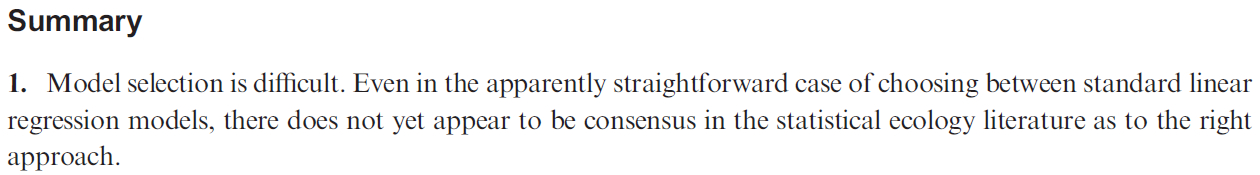
\includegraphics[width=10cm]{graphics/brewer.jpg}\\[2mm]

Note: The first sentence of a paper in \emph{Methods in Ecology and Evolution} from 2016 is: ``Model selection is difficult.''
}

\frame{\frametitle{Mercury example}
Let us look at the mercury example. The {\bf research question} was: \\
``Gibt es einen Zusammenhang zwischen Quecksilber(Hg)-Bodenwerten von Wohnh\"ausern und der Hg-Belastung im K\"orper (Urin, Haar) der Bewohner?''\\[2mm]
\begin{itemize}
\item \emph{Hg concentration in urine} ($Hg_{urine}$) is the {\bf response}.
\item \emph{Hg concentration in the soil} ($Hg_{soil}$) is the {\bf predictor of interest}.\\[5mm]
\end{itemize}

\alert{In addition}, the following variables were monitored for each person, because they might influence the mercury level in a person's body:\\[2mm]

\emph{smoking status; number of amalgam fillings; age; number of monthly fish meals; indicator if fish was eaten in the last 3 days; mother; indicator if vegetables from garden are eaten; migration background; height; weight; BMI; sex; education level.}\\[2mm]

{\bf Thus: In total additional 13 variables!}
}


\frame{\frametitle{How many variables can I include in my model?}

{\bf Rule of thumb:}\\[1mm] 
\colorbox{lightgray}{\begin{minipage}{10cm}
Include no more than $n/10$ (10\% of $n$) variables into your linear regression model, where $n$ is the number of data points.
\end{minipage}}

~\\[2mm]
In the mercury example there are 156 individuals, so a {\bf maximum of 15 variables} should be included in the model.\\[2mm]

{\bf Remarks:}
\begin{itemize}
\item Categorical variables with $k$ levels already require $k-1$ dummy variables. For example, if `education level' has three categories, 2 variables are used up.\\[2mm]
\item Whenever possible, the model should {\bf not be blown up} unneccessarily. Even if there are many data points, the use of too many variables may lead to an {\bf overfitted} model
\end{itemize}
 

}



\frame{
In the mercury study, the following variables were included using \emph{a priori} knowledge:\\[4mm]

\begin{tabular}{llll}
Variable & Meaning & type & transformation\\
\hline
Hg$\_$urin & Hg conc.\ in urine (response) & continuous & $\log$\\ 
Hg$\_$soil & Hg conc.\ in the soil  & continuous & $\log$\\
vegetables & Eats vegetables from garden? & binary\\
migration & Migration background & binary \\
smoking & Smoking status & binary \\
amalgam & No.\ of amalgam fillings & count & $\sqrt{.}$ \\
age & Age of participant &  continuous\\ 
fish & Number of fish meals/month & count  & $\sqrt{.}$\\
last$\_$fish & Fish eaten in last 3 days? &   binary\\
mother & Mother or child?  & binary\\
\end{tabular}
\vspace{2mm}

}

% \frame{Ev list additional variables that were available in the mercury study. \\
% Examples: Height, weight, BMI, sex, the education level (3 categories), the duration of housing in the region (in months).\\[2mm]
% 
% say that no more than 10\% of the number of data points should be used in a model.}


\frame[containsverbatim]{Let us now fit the full model (including all covariates) in R:\\[2mm]


% latex table generated in R 3.3.2 by xtable 1.8-2 package
% Fri Dec 23 12:48:12 2016
\begin{table}[!h]
\centering
\begingroup\footnotesize
\begin{tabular}{rrrr}
  \hline
 & Coefficent & 95\%-confidence interval & $p$-value \\ 
  \hline
Intercept & -0.94 & from -1.10 to -0.79 & $<$ 0.0001 \\ 
  log10(Hg\_soil) & 0.03 & from -0.05 to 0.11 & 0.47 \\ 
  vegetables & 0.079 & from -0.03 to 0.19 & 0.15 \\ 
  migration & -0.048 & from -0.21 to 0.12 & 0.57 \\ 
  smoking & 0.23 & from 0.01 to 0.45 & 0.039 \\ 
  sqrt(amalgam) & 0.36 & from 0.27 to 0.45 & $<$ 0.0001 \\ 
  age & -0.0073 & from -0.02 to 0.01 & 0.32 \\ 
  mother & -0.04 & from -0.50 to 0.42 & 0.86 \\ 
  sqrt(fish) & 0.087 & from 0.03 to 0.14 & 0.003 \\ 
  last\_fish & 0.29 & from 0.13 to 0.44 & 0.0003 \\ 
   \hline
\end{tabular}
\endgroup
\end{table}
\vspace{3mm}
\begin{itemize}
\item There is no evidence that mercury in soil influences mercury in urine ($p=0.47$).\\[2mm]
\item We find $R^2=0.40$. Is this ``good''?\\[2mm]
\item Are there additional terms that might be important?\\[2mm]
\end{itemize}
}

\frame{
Remember from slides 7-10 of week 4 that the dependency of mercury in urine on age is different for mothers and children:

\begin{center}
\setkeys{Gin}{width=0.55\textwidth}
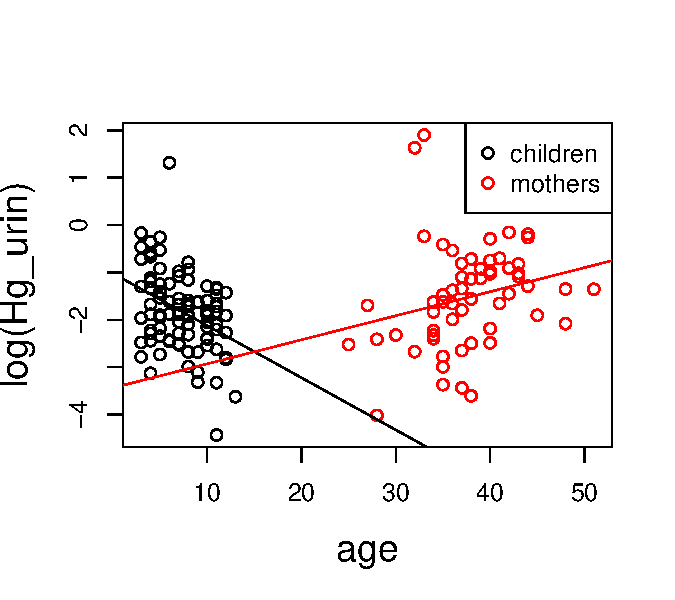
\includegraphics{Bio144_2017_week7-004}
\end{center}

$\rightarrow$ We need to include an interaction term \emph{mother}$\cdot$\emph{age}.
}

\frame[containsverbatim]{\label{sl:mercury_final}
Fitting the model again with the additional term:
% latex table generated in R 3.3.2 by xtable 1.8-2 package
% Fri Dec 23 12:48:12 2016
\begin{table}[!h]
\centering
\begingroup\footnotesize
\begin{tabular}{rrrr}
  \hline
 & Coefficent & 95\%-confidence interval & $p$-value \\ 
  \hline
Intercept & -0.68 & from -0.88 to -0.47 & $<$ 0.0001 \\ 
  log10(Hg\_soil) & 0.033 & from -0.05 to 0.11 & 0.42 \\ 
  vegetables & 0.07 & from -0.03 to 0.17 & 0.18 \\ 
  migration & -0.036 & from -0.19 to 0.12 & 0.65 \\ 
  smoking & 0.27 & from 0.06 to 0.48 & 0.012 \\ 
  sqrt(amalgam) & 0.33 & from 0.24 to 0.42 & $<$ 0.0001 \\ 
  age & -0.042 & from -0.06 to -0.02 & 0.0004 \\ 
  mother & -1.03 & from -1.70 to -0.35 & 0.003 \\ 
  sqrt(fish) & 0.079 & from 0.03 to 0.13 & 0.004 \\ 
  last\_fish & 0.30 & from 0.15 to 0.45 & $<$ 0.0001 \\ 
  age:mother & 0.055 & from 0.03 to 0.08 & 0.0002 \\ 
   \hline
\end{tabular}
\endgroup
\end{table}
\vspace{3mm}
\begin{itemize}
\item There is evidence that the interaction is relevant ($p<0.001$).\\[2mm]
\item $R^2$ has now clearly increased to $0.45$.\\[2mm]
\end{itemize}

$\rightarrow$ The interaction term apparently improved the model.
}

\frame[containsverbatim]{
A model checking step (always needed, but we did it already in weeks 4)
\setkeys{Gin}{width=0.8\textwidth}
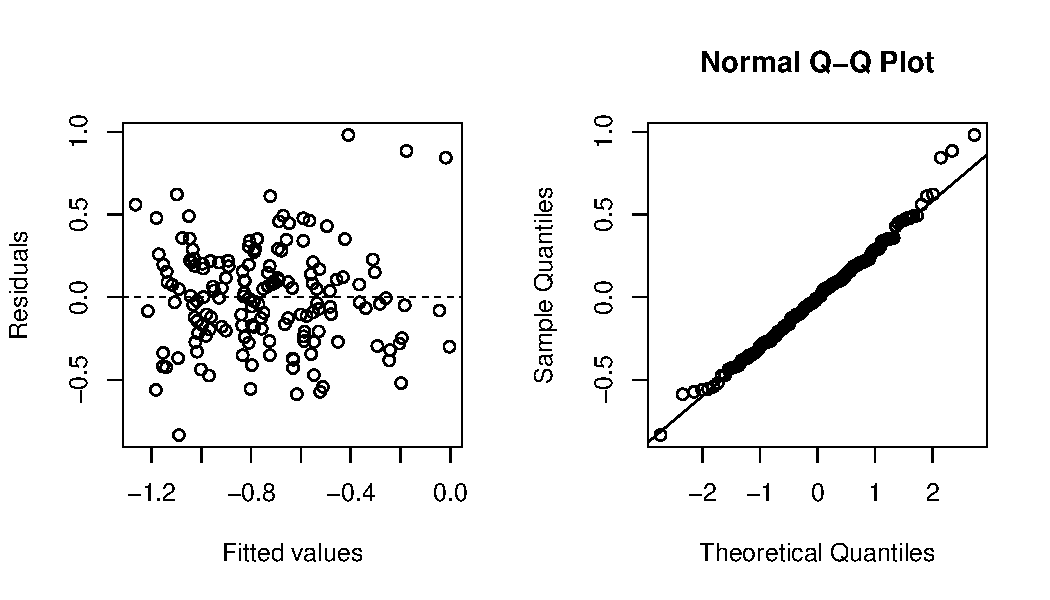
\includegraphics{Bio144_2017_week7-modelChecksHg}
\vspace{2mm}

This looks ok, no need to improve the model from this point of view.
}

\frame{
Even if the model checking step revealed no violations of the assumptions (the model seems to be fine), we sometimes want to know:\\[2mm]

\begin{itemize}
\item Which of the terms are \alert{important/relevant}?\\[2mm]
\item Are there \alert{additional terms} that might be important?\\[2mm]
\item Would it be possible to further \alert{``improve'' the model}?\\[3mm]
\end{itemize}
\vspace{3mm}

Often, the desire is to find a model that is in some sense ``optimal'' or ``best''.  
}


\frame{\frametitle{Is importance reflected by $p$-values?}
A widely used practice to determine the ``importance'' of a term is to look at the $p$ value from the $t$-test and check if it falls below a certain threshold (usually $p<0.05$). \\[4mm]

{\bf However, there are a few problems with this approach:}\\[2mm]

\colorbox{lightgray}{\begin{minipage}{10cm}
\begin{itemize}
\item {\bf A small $p$-value does not necessarily mean that a term is (biologically, medically) important -- and vice versa!}\\[2mm]
\item When carrying out the $t$-tests with $H_0: \beta_j=0$ for all variables , one runs into a \alert{multiple testing problem}.\\
{(\scriptsize Remember the ANOVA lecture, week 5, slide 25).}\\[2mm]
\item The respective tests depend crucially on the correctness of the \alert{normality assumption}.\\[2mm]
\item Covariates are sometimes \alert{collinear}, which leads to more uncertainty in the estimation of the respective regression parameters, and thus to larger $p$-values.\\[2mm]
\end{itemize}
\end{minipage}}
}

\frame{
For all these reasons, we {\bf strongly disagree} with the remark in Stahel's script 5.2, second part in paragraph d.\\[4mm]

The first part is ok:\\[2mm]

\includegraphics[width=10cm]{graphics/52d_1.pdf}\\[2mm]

But we disagree with this:\\[2mm]

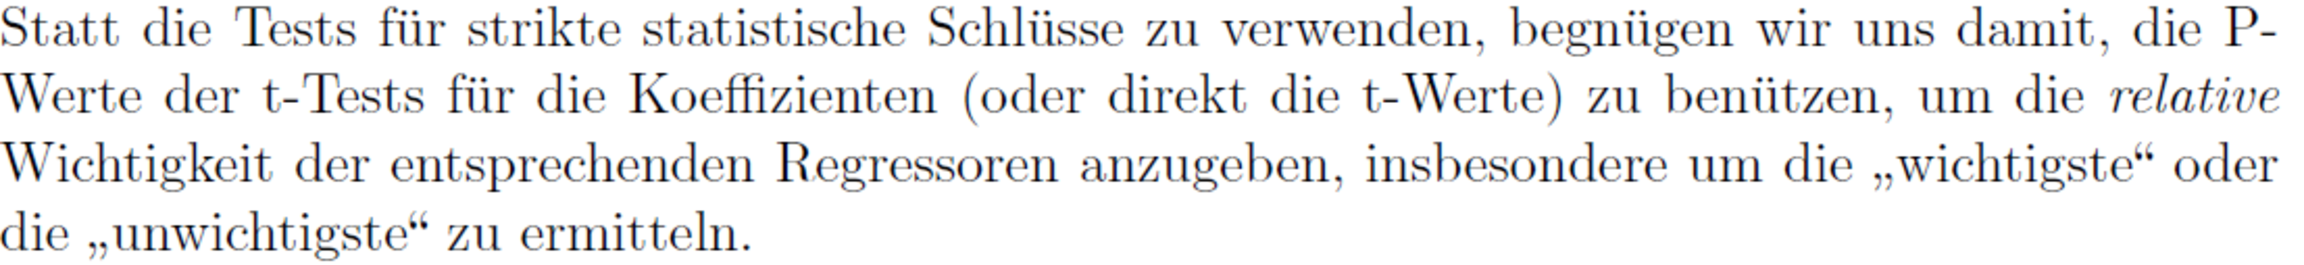
\includegraphics[width=10cm]{graphics/52d_2.pdf}
}


\frame{\frametitle{Automatic model selection procedures}
It would be very convenient if there were {\bf objective} or even {\bf automatic} procedures to select the ``best'' model. Wouldn't it?\\[2mm]

In fact, such procedures have been proposed in the past. For example:\\[4mm]
\begin{itemize}
\item \alert{Forward selection:}\\
Start with a large/full model. In each step, remove the variable with the largest $p$-value. Do this until only variables with low $p$-values remain in the model.\\[4mm]
\item \alert{Backward selection:}\\
Start with an empty model. In each step, add the predictor with the highest importance (lowest $p$-value). Do this until none of the missing coefficients has a low $p$-value when adding it.\\[2mm]
\end{itemize}


}


\frame[containsverbatim]{\frametitle{Model selection bias}
Let us reproduce an illustrative example that was described by \citet{freedman1983}. \\[2mm] 

{\bf Aim of the example:} \\[2mm]
\colorbox{lightgray}{\begin{minipage}{10cm}
To illustrate how model selection purely based on $p$-values can lead to biased parameters and overestimated effects.
\end{minipage}}
\vspace{2mm}

Procedure:
\begin{enumerate}
\item \alert{Randomly generate} 100 data points for 50 covariables $\bm{x}^{(1)},\ldots, \bm{x}^{(50)}$ and a response $\bm{y}$: \\[4mm]

\begin{Schunk}
\begin{Sinput}
> set.seed(9856)
> data <- data.frame(matrix(rnorm(51*100),ncol=51))
> names(data)[51] <- "Y"
\end{Sinput}
\end{Schunk}
\vspace{1mm}

\texttt{data} is a 100$\times$ 51 matrix, where the last column is the response. The \alert{data were generated completely independent}, the covariates do not have any explanatory power for the response! 
\end{enumerate}
}

\frame[containsverbatim]{
\begin{enumerate}
\setcounter{enumi}{1}
\item Fit a linear regression model of $\bm{y}$ against all the 50 variables
\begin{equation*}
y_i = \beta_0 + \beta_1 x_i^{(1)} + \ldots + \beta_{50}x_i^{(50)} + e_i \ .
\end{equation*}
\begin{Schunk}
\begin{Sinput}
> r.lm <- lm(Y~.,data)
\end{Sinput}
\end{Schunk}

As expected, the distribution of the $p$-value is (more or less) uniform between 0 and 1:\\
\setkeys{Gin}{width=0.5\textwidth}
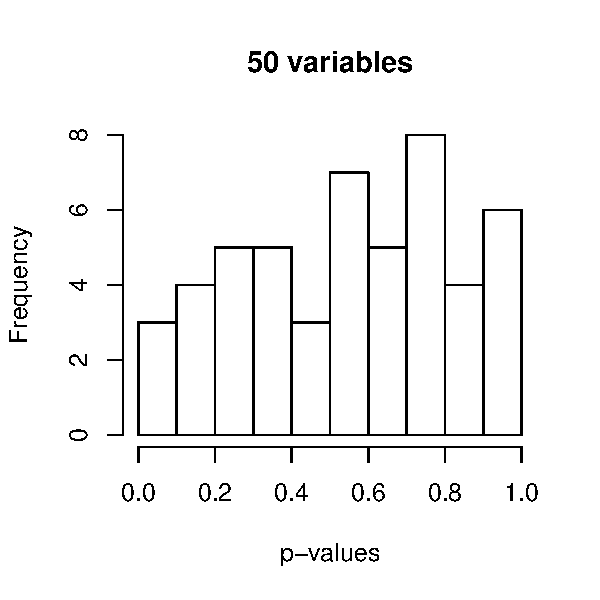
\includegraphics{Bio144_2017_week7-010}

\end{enumerate}
}

\frame[containsverbatim]{
\begin{enumerate}
\setcounter{enumi}{2}
\item Then pick all variables that have a $p<0.25$ and re-fit the model using only these. 11 variables fulfil this criterion:\\[2mm]
\begin{Schunk}
\begin{Sinput}
> # select all variables with p<0.25
> r.lm.red <- lm(Y ~ X1 + X2 + X4 + X5 + X14 + X18 + X20 + X27 + X36 + X38 + X49,data)
\end{Sinput}
\end{Schunk}


\setkeys{Gin}{width=0.5\textwidth}
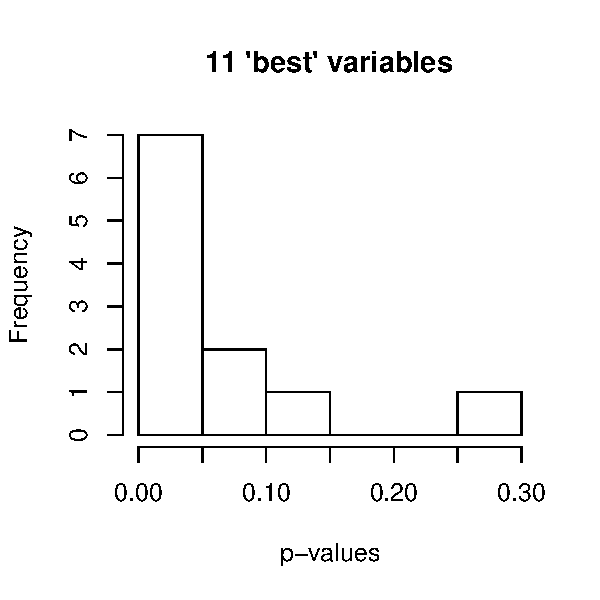
\includegraphics{Bio144_2017_week7-012}

The distribution of the $p$-values is now skewed: many of them reach ``significant'' values (7 have $p<0.05$). This happened \alert{although none of the variables has any explanatory power!}
\end{enumerate}
}



\frame{\frametitle{Important note}
\colorbox{lightgray}{\begin{minipage}{10cm}
{\bf Automatic model selection procedures may lead to biased parameter estimates and wrong conclusions!}
\end{minipage}}
{\scriptsize See, e.g., \citet{freedman1983, copas1983}.}
\vspace{6mm}

Please note that {\bf we therefore strongly discourage the use of automated model selection procedures}. So please ignore large parts of chapter 5.3 in the Stahel script!! \\[2mm]

(Or read it to see how you should {\bf not} do it.)
}

\frame{\frametitle{More modern ways to do model selection}

\underline{Remember:} $R^2$ is not suitable for model selection, because it \emph{always} increases (improves) when a new variable is included.\\[4mm] 

In 2002, Burnham and Anderson suggested the use of so-called \alert{information-criteria} for model selection. \\[4mm]

The idea is to find a \alert{balance between}\\[4mm]

\begin{center}
{\bf Good model fit} $\quad\leftrightarrow\quad$ {\bf Low model complexit}
\end{center}

~\\[4mm]
$\rightarrow$ Penalize models with more parameters.
}

\frame{\frametitle{AIC}
The most prominent criterion is the \alert{AIC (Akaike Information Criterion)}, which measures the \alert{quality of a model}.\\[4mm]

\colorbox{lightgray}{\begin{minipage}{10cm}
The AIC of a model with likelihood $L$ and $p$ parameters is given as
\begin{equation*}
AIC = -2\log(L) + 2p \ .
\end{equation*}
\end{minipage}}

~\\[4mm]
{\bf Important: The \underline{lower} the AIC, the \underline{better} the model!}\\[6mm]

The AIC is a \alert{compromise} between
\begin{itemize}
\item a high likelihood $L$ (good model fit) 
\item few model parameters $p$ (low complexity)
\end{itemize}


}

\frame{\frametitle{AIC$_c$: The AIC for low sample sizes}
When the number of data points $n$ is small with respect to the number of parameters $p$ in a model, the use of a \alert{corrected AIC, the AIC$_c$} is recommended.\\[2mm]

\colorbox{lightgray}{\begin{minipage}{10cm}
The {\bf corrected AIC} of a model with $n$ data points, likelihood $L$ and $p$ parameters is given as
\begin{equation*}
AIC_c = -2\log(L) + \frac{2p(p+1)}{n-p-1} \ .
\end{equation*}
\end{minipage}}
~\\[4mm]

Burnham and Anderson {\bf recommend to use AIC$_c$ in general, but for sure when the ratio $n/p<40$.}\\[2mm]

In the \alert{mercury example}, we have 156 data points and 11 parameters (including the intercetp $\beta_0$), thus $n/p = 156/11 \approx 14 <40$ $\Rightarrow$ AIC$_c$ should be used! 
}

\frame{\frametitle{BIC, the brother of AIC}
Other information criteria were suggested as well. Another prominent example is the \alert{BIC (Bayesian Information Criterion)}, which is similar in spirit to the AIC. \\[2mm]

\colorbox{lightgray}{\begin{minipage}{10cm}
The BIC of a model for $n$ data points with likelihood $L$ and $p$ parameters is given as
\begin{equation*}
BIC = -2\log(L) + p \cdot \ln(n) \ .
\end{equation*}
\end{minipage}}

~\\[4mm]
{\bf Again: The \underline{lower} the BIC, the \underline{better} the model!}\\[6mm]

The only difference to AIC is the complexity penalization. The BIC criterion is often {\bf claimed to estimate the predictive quality} of a model. More recent research indicates that AIC and BIC perform well under different data structures \citep{brewer.etal2016}.\\[2mm]
}

\frame{
\colorbox{lightgreen}{\begin{minipage}{10cm}
Don't worry: No need to remember all these AIC and BIC formulas by heart!
\end{minipage}}

\vspace{8mm}
What you should remember: \\[2mm]

AIC, AIC$_c$ and BIC all have the {\bf aim to find a good quality model by penalizing model complexity}.
}

\frame[containsverbatim]{\frametitle{Example of AIC use}
\vspace{-10mm}
{\scriptsize (Essentially the same as BIC use.)}\\[4mm]

Remember that we first fitted the mercury example {\bf without} (\texttt{r.lm1}) and {\bf with} (\texttt{r.lm2}) the interaction $mother\cdot age$. The model improvement is also confirmed by the {\bf reduction in AIC$_c$} (which we used because $n/p<40$):\\[6mm]

\begin{Schunk}
\begin{Sinput}
> library(AICcmodavg)
> AICc(r.lm1)
\end{Sinput}
\begin{Soutput}
[1] 109.2942
\end{Soutput}
\begin{Sinput}
> AICc(r.lm2)
\end{Sinput}
\begin{Soutput}
[1] 96.66951
\end{Soutput}
\end{Schunk}
~\\[6mm]
\underline{Interpretation:} The AIC$_c$ of the model with interaction is clearly lower, thus the model with interaction is to be preferred.\\[4mm]

}

\frame[containsverbatim]{\label{sl:migration}
We can further play around with AIC and, for instance, fit a model withouth the binary \emph{migration} variable:\\[4mm]

\begin{Schunk}
\begin{Sinput}
> r.lm3 <- lm(log10(Hg_urin) ~ log10(Hg_soil) + vegetables  + smoking + 
+              sqrt(amalgam) + age * mother + sqrt(fish) + last_fish,d.hg)
> AICc(r.lm3)
\end{Sinput}
\begin{Soutput}
[1] 94.53696
\end{Soutput}
\end{Schunk}

~\\[4mm]
\underline{Interpretation:} We observe a further reduction of the AIC. \\[4mm]

This ``success'' brings us to another idea:\\[2mm]
\colorbox{lightgray}{\begin{minipage}{10cm}
{\bf Could we do model selection simply by minimizing the AIC?}\\
Without actually ``thinking''?
\end{minipage}}
}

\frame{\frametitle{Model selection with AIC?}

Given $m$ potential variables to be included in a model.\\[2mm]

\begin{itemize}
\item In principle it is possible to minimize the AIC over all $2^m$ possible models. Simply fit all models and take the ``best'' one (lowest AIC).\\[2mm]
\item Sometimes the best few models have very similar AIC. It is then possible to do {\bf model averaging}, e.g.\ over the best 3 models, by weighting them according to the AIC (not done in this course).\\[6mm]
\end{itemize}

{\bf However:}
\begin{itemize}
\item As always when one tries to circumvent ``thinking'', this may lead to unreasonable models.\\[2mm]
\item AIC is in some sense equivalent to $p$-values-based statistics for {\bf nested models} (i.e., when the smaller model contains a subset of the larger model).
\end{itemize}
}


\frame{\frametitle{Predictive and explanaory models}

Before we continue to discuss model selection, let us introduce an important discrimination between models that aim at explanation and those that aim at prediction:\\[2mm]

\begin{itemize}
\item \alert{\bf Explanatory models}: These are models that aim to understand the (causal) relationship between covariates and the response. \\
\underline{Example:} The mercury study aims to understand if Hg-concentrations in the soil (covariable) influence the Hg-concentrations in humans (response).\\[2mm]

\item \alert{\bf Predictive models}: These are models that aim to predict the outcome of future subjects.\\
\underline{Example:} In the bodyfat example the aim is to predict people's bodyfat from factors that are easy to measure (age, BMI, weight,..).
\end{itemize}

~\\
\colorbox{lightgray}{\begin{minipage}{10cm}
{\bf Please note:} The model selection strategy depends on this distinction.
\end{minipage}}
}

\frame{\frametitle{Prediction vs explanation}
\colorbox{lightgray}{\begin{minipage}{10cm}
When the aim is \emph{prediction}, the best model is the one that best predicts the fate of a future subject. This is a well defined task and automatic strategies to find the model which is best in this sense are potentially useful. \\[4mm]

However, when used for \emph{explanation} the best model will depend on the scientific question being asked, {\bf and automatic selection strategies have no place}. 
\end{minipage}}\\[5mm]

{\scriptsize\citep{clayton.hills1993}}

}


\frame{\frametitle{Your aim is prediction?}
 
Ideally, the predictive ability of a model is tested by a cross-validation (CV) approach, but
AIC, AIC$_c$, BIC are useful approximations to CV.\\[4mm]  
 
Automatic model selection procedures using criteria like AIC, AIC$_c$, BIC may threfore be useful.\\[4mm]


\vspace{4mm}
\href{https://en.wikipedia.org/wiki/Cross-validation_(statistics)}
{\beamergotobutton{Find a description of the CV idea here.}}
}


\frame{\frametitle{Your aim is explanation?}  

{\bf Then please select your covariates according to \emph{a priori} knowledge.}\\[6mm]

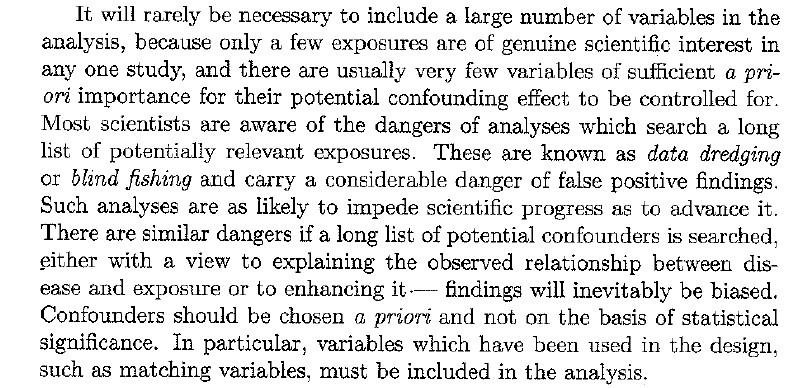
\includegraphics[width=10.5cm]{graphics/claytonHills.jpg}\\
{\scriptsize\citep{clayton.hills1993}}
}

\frame{\frametitle{Correct way of model selection for explanatory models}

Automatic model selection strategies are thus {\bf not recommended for explanatory models} (example: mercury study). We therefore recommend the following steps:\\[2mm]

\begin{itemize}
\item {\bf Think about a suitable model \alert{before} you start}. This includes the model family (e.g., linear model), but also potential variables that are relevant using \emph{a priori} knowledge.\\[2mm]
\item After fitting the model, \alert{check if modelling assumptions are met}.\\[2mm]
\item If modelling assumptions are not met, {\bf try to find out why and adapt the model}.  
  \begin{itemize}
  \item Is a transformation of variables needed? 
  \item Wrong model family (e.g., linear regression is not suitable)?
  \item Are terms missing in the model?
  \item Outliers?
  \item ... 
  \end{itemize}
\item Interpret the model coefficients (effect sizes) and the $p$-values properly (see next week).
\end{itemize}

}

\frame[containsverbatim]{\frametitle{Final comments on the mercury example}
Given that the mercury model is an {\bf explanatory models}, we should not remove a variable (e.g., migration) simply because it reduces AIC (see slide \ref{sl:migration}).\\[2mm]

Therefore, given the a priori selection of variables and the model validation results, the model from slide \ref{sl:mercury_final} was used in the final publiation (give reference here).
}


\frame{\frametitle{Occam's Razor principle}

The principle essentially says that an explanatory model should not be made more complicated than necessary.\\[4mm]

This is also known as the \alert{principle of {\bf parsimony}}:\\[4mm]

\colorbox{lightgray}{\begin{minipage}{10cm}
Systematic effects should be included in a model {\bf only} if there is convincing evidence for the need of them.
\end{minipage}}

\vspace{4mm}
\href{https://de.wikipedia.org/wiki/Ockhams_Rasiermesser}
{\beamergotobutton{See Wikipedia for ``Ockham's Rasiermesser''}}
}



\frame[containsverbatim]{\frametitle{The bodyfat example}
The bodyfat study is a typical example for a {\bf predictive model}.\\[2mm] 

There are 12 potential predictors (plus the response). Let's fit the full model:\\[2mm]



\begin{Schunk}
\begin{Sinput}
> r.bodyfat <- lm(bodyfat ~ ., d.bodyfat)
\end{Sinput}
\end{Schunk}

% latex table generated in R 3.3.2 by xtable 1.8-2 package
% Fri Dec 23 12:48:13 2016
\begin{table}[!h]
\centering
\begingroup\footnotesize
\begin{tabular}{rrrr}
  \hline
 & Coefficent & 95\%-confidence interval & $p$-value \\ 
  \hline
Intercept & -115.96 & from -228.65 to -3.26 & 0.044 \\ 
  age & 0.02 & from -0.04 to 0.08 & 0.52 \\ 
  gewicht & -0.76 & from -1.46 to -0.07 & 0.032 \\ 
  hoehe & 0.58 & from -0.04 to 1.21 & 0.068 \\ 
  bmi & 2.48 & from 0.26 to 4.70 & 0.029 \\ 
  neck & -0.60 & from -1.04 to -0.16 & 0.008 \\ 
  chest & -0.14 & from -0.37 to 0.08 & 0.20 \\ 
  abdomen & 0.92 & from 0.74 to 1.11 & $<$ 0.0001 \\ 
  hip & -0.31 & from -0.61 to -0.01 & 0.046 \\ 
  thigh & 0.25 & from -0.05 to 0.55 & 0.11 \\ 
  knee & 0.073 & from -0.43 to 0.58 & 0.78 \\ 
  ankle & -0.49 & from -1.17 to 0.19 & 0.15 \\ 
  biceps & 0.17 & from -0.16 to 0.49 & 0.32 \\ 
   \hline
\end{tabular}
\endgroup
\end{table}}

\frame[containsverbatim]{
Given the predictive nature of the model, we do some automatic model selection for this dataset, for instance using the \texttt{stepAIC()} function from the \texttt{MASS} package:\\[6mm]

\begin{Schunk}
\begin{Sinput}
> library(MASS)
> # model with optimal AIC:
> r.AIC <- stepAIC(r.bodyfat, direction = c("backward"), trace = FALSE)
> AIC(r.bodyfat)
\end{Sinput}
\begin{Soutput}
[1] 1412.148
\end{Soutput}
\begin{Sinput}
> AIC(r.AIC)
\end{Sinput}
\begin{Soutput}
[1] 1407.521
\end{Soutput}
\end{Schunk}
~\\[6mm]

$\rightarrow$ The AIC for the optimal model is $1407.5$, compared to the full model with an AIC of $1412.1$. This is not a very dramatic improvement.
}

\frame[containsverbatim]{
But at least the model was now reduced, and only 8 of the 12 variables remain in the model:\\[2mm]

% latex table generated in R 3.3.2 by xtable 1.8-2 package
% Fri Dec 23 12:48:14 2016
\begin{table}[!h]
\centering
\begingroup\footnotesize
\begin{tabular}{rrrr}
  \hline
 & Coefficent & 95\%-confidence interval & $p$-value \\ 
  \hline
Intercept & -112.87 & from -222.74 to -2.99 & 0.044 \\ 
  gewicht & -0.75 & from -1.42 to -0.07 & 0.031 \\ 
  hoehe & 0.53 & from -0.09 to 1.15 & 0.091 \\ 
  bmi & 2.17 & from 0.01 to 4.33 & 0.049 \\ 
  neck & -0.54 & from -0.97 to -0.11 & 0.014 \\ 
  abdomen & 0.91 & from 0.76 to 1.06 & $<$ 0.0001 \\ 
  hip & -0.29 & from -0.58 to 0.00 & 0.05 \\ 
  thigh & 0.30 & from 0.04 to 0.56 & 0.023 \\ 
  ankle & -0.45 & from -1.09 to 0.18 & 0.16 \\ 
   \hline
\end{tabular}
\endgroup
\end{table}~\\[3mm]

{\bf Note:}  AIC minimization may lead to a model that retains variables with relatively large $p$-values (e.g., ankle).\\[2mm]
{\bf Again:} Such a procedure should not be applied for an explanatory model. Moreover, the coefficients should not be (over-)interpreted.
}




\frame{\frametitle{Summary}

}

\frame{\frametitle{Reading and exercises for the self-study week}
\begin{itemize}
\item Paper by \citet{freedman1983}
\item 
\end{itemize}
}

\frame{References:
\bibliographystyle{Chicago}
\bibliography{refs}
}



\end{document}
